%!TEX root = thesis.tex

\chapter{A population of ``clumpy'' galaxies in local Universe}\label{chap:5}
Simultaneous to the development of this research was the publishing of the Galaxy Zoo: Hubble galaxy classification catalog. A portion of the original GZ2 SDSS galaxy sample was included in Galaxy Zoo: Hubble because the decision tree for the latter was more complex than that for GZ2. This enabled a comparison between different decision trees and led to the identification of a rare sample of extremely low redshift clumpy galaxies. This chapter details the identification of such a sample, preliminary analysis of the star-forming clumps, and methods to identify more such galaxies in the local universe as these may be analogs of high redshift galaxies with similar properties.

\section{Introduction}
Structural properties of typical galaxies today wereforgedover the5billionyearsbetween the peakof the cosmic star-formation history at z ⇠ 1.5  2 and now.From the theoretical perspective,galaxies’ growth is predominantly governed by the baryonic physics of gas accre-tion and energy feedback, rather than by merg-ers that induce starbursts (e.g., Somerville and Dav ́ e, 2015). Gas inflow modulates galaxies’ star formation history and plays a crucial role in the dynamical state of the galaxy.A varying gas fraction changes the amount of fragmentation within the gaseous disk, the star-formation rates (SFR), strengths and lifetimes of disk structural components, and possibly the fueling rate of the AGN. As a consequence of the gas accretion pro-cess, the small-scale structure within disk galax-ies is also predicted to change over time, with the appearance of stable “grand design” spiral arms only at later epochs (e.g. Oppenheimer et al., 2010; Bouch ́ e et al., 2010; Dav ́ e et al., 2011a,b; Lilly et al., 2013; Hirschmann et al., 2013). 

n the theoretical paradigm discussed above, the origin of these massive clumps is still an open debate. Two main physical scenarios have been proposed.On one side (hereafter referred to as in-situ models),giant clumps are expectedto form inside pre-existing galaxies.In these sce-narios, haloes located at the center of multiple filaments continuously accrete gas from the cos-mic web.This accretion results in the forma-tion of gas-dominated disks that eventually frag-ment into giant clumps by gravitational insta-bility (Bournaud et al., 2007; Dekel et al., 2009; Behrendt et al., 2015). On the other side (here-after referred to as ex-situ models) clumps may have an external origin, as in the case of mergers with small star-forming companions (Ceverino et al., 2010; Bournaud, 2016). 

Observationally, the situation is still unclear. The large gas-to-baryonic fraction of 20 to 80 recently measured with interferometric studies in clumpy galaxies lends support to the in-situ models(e.g., Erb et al., 2006; Tacconi et al., 2008, 2010).Similarly, the kinematics in the majorityofthesegalaxiesischaracterized by large, regularly-rotating disks, with no signs of on-going or recent mergers (Genzel et al., 2006; F ̈ orster Schreiber et al., 2009; Epinat et al., 2012; Newman et al., 2012).These studies, however, are 1) limited to galaxies with SFR> 10M yr 1 and M>10 10 M) and 2) include only a few galaxies with high spatial resolution kinematic and interferometric data (Genzel et al., 2014). 

The lack of existing observational constraints below 10 10 M is of particular concern. It is pre-cisely in this mass range that most of the con-straining power resides. In fact, state of the art simulations that directly resolve the interstellar medium of individual galaxies while capturing their cosmological environment show that low mass galaxies are the mostly a↵ected by preven-tive feedback (e.g., FIRE Muratov et al.2015; 11
GASOLINE Christensen et al. 2015; and MU-FASA Dav ́ e et al.2016).These simulations show that in galaxies with M<10 10 supernova-driven fast outflows can lower the gas inflow rate, and consequently the rate at which clumps are formed in-situ, compared to more massive galax-ies. If clumps are the result of minor merging, on the other hand, the dependency with stellar mass would depend on the specifics of the dy-namics of the mergers. 

\section{Sample Selection \& Data} \label{sec:chap5-sample}
We identify a sample of clumpy galaxies in the local universe by considering classifications from both the Galaxy Zoo 2 (GZ2) \citep{Willett2013} and Galaxy Zoo: Hubble (GZH) \citep{Willett2017} projects. We provide a brief overview of each of these projects here. 

The GZ2 subject sample consists of 285,962 galaxies identified as the brightest 25\% ($r$-band magnitude $< 17$) residing in the SDSS North Galactic Cap region from Data Release 7 and included subjects with both spectroscopic and photometric redshifts out to $z < 0.25$. In addition to the DR7 Legacy catalog, galaxies were included from Stripe 82, a multipy-imaged strip along the celestial equator in the Southern Galactic Cap. Galaxies in this region were selected to have $m_r\le17.7$ and petror90\_r $>3$, where petror90\_r is the radius containing 90\% of the r-band Petrosian aperture flux.

The GZH project contains images drawn from several dedicated surveys and sample selection criteria. Most samples are drawn from various Hubble fields such as AEGIS, GOODS and COSMOS; however also included are the single-epoch and co-added images from Stripe 82 of the SDSS Data Release 7 that were part of the GZ2 project. The single-epoch imaging allows for local comparison to higher redshift galaxies, while the co-added imaging allows for image depth analyses. 

The most notable difference between these two projects is the decision tree presented to volunteers. The goal of GZH was to collect detailed morphologies for galaxies in Hubble imaging which extends to much higher redshift than those of the SDSS sample. Galaxies at higher redshift do not necessarily follow the traditional Hubble sequence and thus a new branch of questioning was added to the decision tree for this project, shown in Figure \ref{fig: gzh decision tree}. This included several questions concerning the clumpy nature of galaxies, a morphological feature well known to exist at higher redshift. Because GZH included galaxies from the GZ2 project, we can draw on both sets of decision trees to identify clumpy features for galaxies in Stripe 82.

\begin{figure}
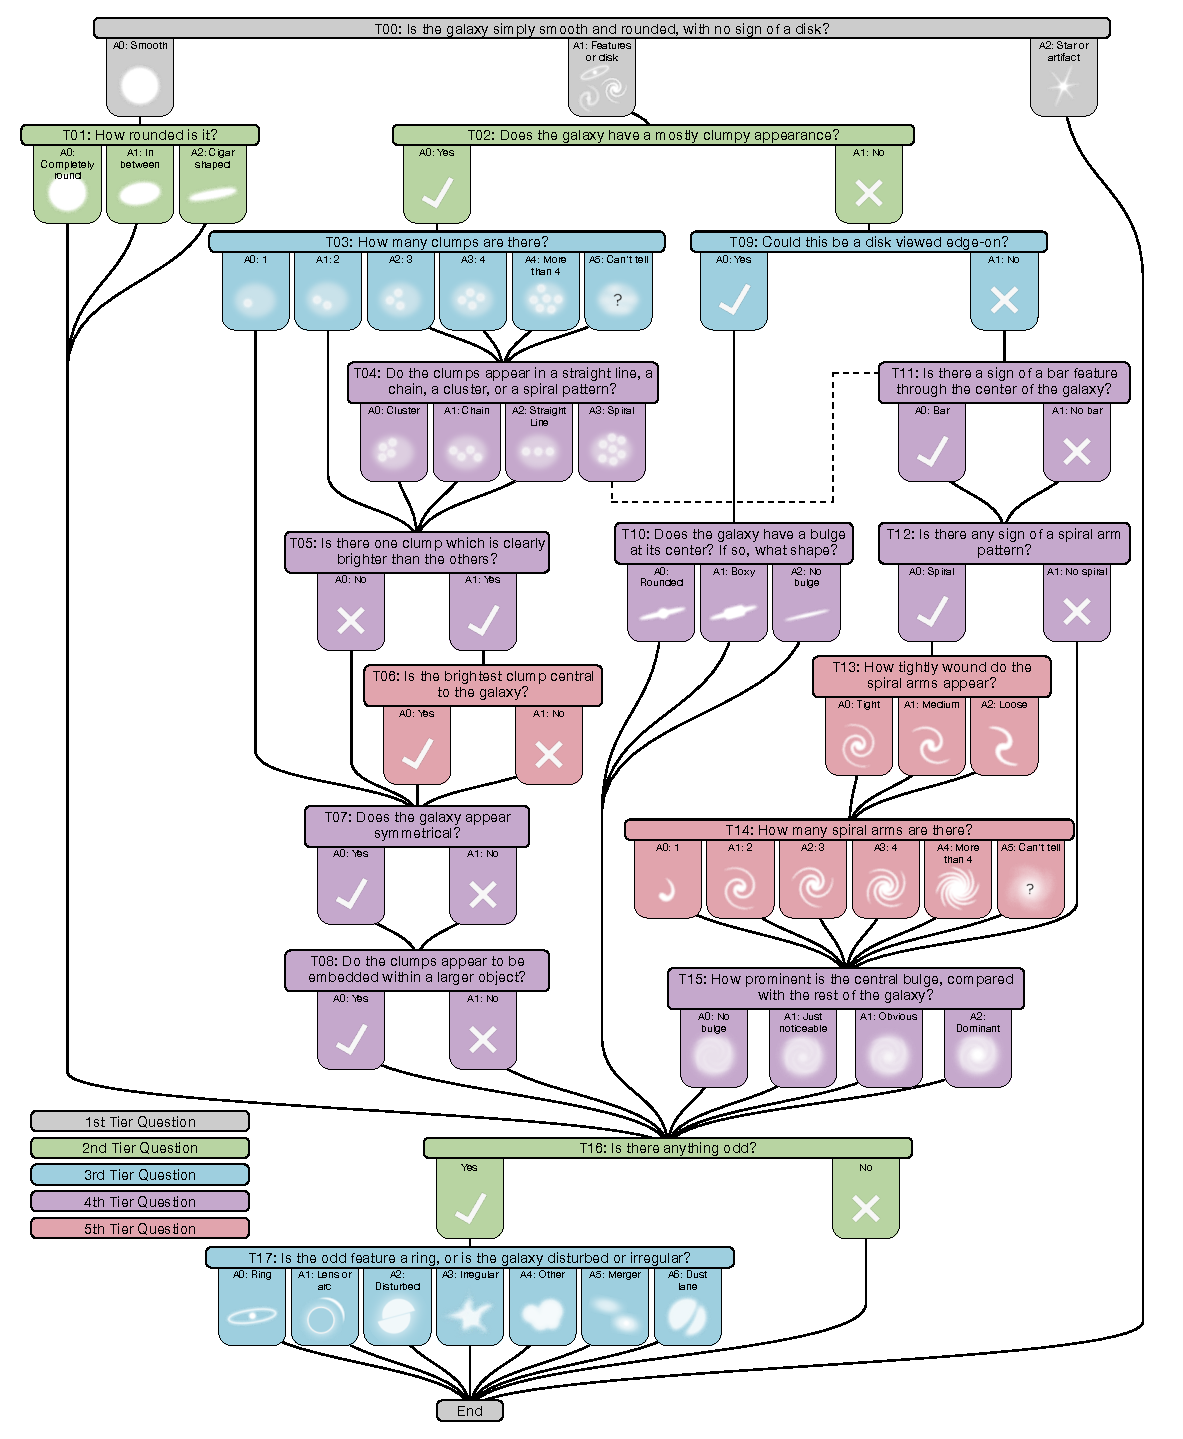
\includegraphics[width=\textwidth]{Figures/gz3_tree_resized.pdf}
\caption[Galaxy Zoo: Hubble decision tree.]{Galaxy Zoo: Hubble decision tree. The most notable difference between this decision tree and that used during the Galaxy Zoo 2 project is the ``clumpy'' branch of tasks.}
\label{fig: gzh decision tree}
\end{figure}


To select a sample of ``clumpy" galaxies from the GZH Stripe 82 sample, we consider only those subjects with large featured (\ffeat) and clumpy (\fclump) vote fractions: the fraction of volunteers who voted a subject as `featured or disk' in response to the first question ``Is the galaxy simply smooth and rounded, with no sign of a disk?'' and who answered `yes' to the question ``Does the galaxy have a mostly clumpy appearance?'' Specifically, we select galaxies which satisfy \ffeat~$\ge0.5$ and \fclump~$\ge0.5$ Additionally, we require $N_{\mathrm{votes}} \ge 20$, where $N_{\mathrm{votes}}$ is the number of volunteers who answerd the clumpy question. This insures that \fclump~is statistically significant and not a product of too few votes.  This yields a sample of 629 galaxies: 273 single-epoch imaging and 356 from the co-added imaging. After visual inspection we find that this is hardly a pure sample of clumpy galaxies in the traditional sense, instead including a sizeable sample of tight groups of elliptical galaxies, as well as galaxies in various merging states, possessing multiple nuclei. [\textbf{show example image?}] After excluding these and duplicate imaging, we retain 92 coadd-depth and 105 single-depth clumpy galaxies, of which 156 are unique systems (some objects are common to both the single-epoch and coadd-depth imaging). Finally, we exclude galaxies with $z>0.06$ in order to retain a sample wherein the physical scale as observed by SDSS is similar to Hubble's at $z\sim3$ to allow for comparison with high redshift samples. Our final sample contains 105 unique galaxies. 


We obtain SDSS Data Release 12 (DR12) \textit{ugriz} coadd imaging, as well as all optical spectra associated with each galaxy. The wavelength range of the SDSS spectra is $3800-9200$\AA~with a resolution of $R\sim 1500$ at $\sim3800$\AA. The $3$\arcsec~SDSS fibers cover 2.9 kpc at $z=0.05$. We visually inspect these spectra to verify that the fiber was positioned over a star-forming region rather than the galactic bulge or other structure. Through this inspection we determine that one clumpy galaxy is actually a juxtoposition of three galaxies at disparate redshifts flagged as clumpy in GZH due to the low resolution of SDSS imaging. We exclude this subject from our sample. Our final list includes 175 spectra. Approximately half of the galaxies in our sample have more than one spectrum with a handful having three or four spectra.  
 
%The physical scale at z= 0.06 is 1"=1.1kpc. SDSS pixel scale is 0.396"/pixel. --> 0.43 kpc/pixel -->  ~2.3 pixels = 1kpc.  


\section{Analysis}
During visual inspection of galaxy images we discover that the SDSS pipeline assigns central galactic coordinates incorrectly, likely due to these galaxies having low overall surface brightness with several bright clumps. The clumps are often marked as individual objects by the SDSS pipeline but, to the human eye, are obviously part of a larger system. As we need to determine accurate photometry and stellar masses for these galaxies we thus reevaluate their isophotal areas. We create postage stamps of each galaxy for all \textit{ugriz} SDSS fields.  Where possible, the size of the postage stamp is taken to be five times $\mathtt{petrorad\_r}$, the Petrosian radius as measured in the $r$-band by the SDSS pipeline. However, for those galaxies which are improperly measured, we create the cutout by eye to include the full extent of the galactic light profile. 

We next process the $r$-band (maybe g-band cuz that's more blue?) postage stamp with Source Extractor (Bertin and whoever) using parameters designed to detect low surface brightness features. Important parameters are detailed in Table X that doesn't exist yet. Though these parameters adequately identify most of our sample, galaxies that fail are redone individually and SE parameters are tweaked for each particular case. These segmentation maps define the galaxy extent for all future analysis. 



\subsection{Measuring clump radial distance} \label{subsec:radii}


\subsection{Clump Halpha Hbeta ratios [Dust]} \label{subsec:dust}

\subsection{Clumpy Halpha equivalent widths} \label{subsec:ew}




%% If you wish to include an acknowledgments section in your paper,
%% separate it off from the body of the text using the \acknowledgments
%% command.

\section{Clump Scout}
Discuss the SDSS non-Stripe 82 sample -- since it was not included in GZH there is no information about the clumpiness of these galaxies. However, because we find a substantial sample in Stripe 82, this motivates an additional pass of the rest of GZ2's galaxy sample to find more. 

We choose a subset of GZ2 non-Stripe 82 galaxies for clumpy examination. They must be low redshift ($z\le0.06$) and with \fsmooth~$\le0.8$ to exclude those galaxies which are obviously elliptical and thus would not have travelled down the clumpy track of the GZH decision tree. These criteria yield a sample of $\sim45$K galaxies. 

Describe the project: We would ask only the top-level clumpy question from the GZH decision tree: ``Does the galaxy have a mostly clumpy appearance?'' If volunteers respond in the affirmative, a second task will ask them to identify the location of these clumps by using the Zooniverse point tool: a drag and drop circle which can be placed anywhere on the image and sized according to fit the clump within the confines of the circle. 

The goal of this project is to identify additional low redshift galaxies with bright star-forming clumps. This will allow multiple avenues of study: determining the fraction of clumpy galaxies in the local universe, a task which today is quite difficult and at this low redshift has very large error bars -- cite who?? Guo?? And the other one which I forgot. Go find the NSF proposal!

In order to secure reliable measurements for \fclump~in the local universe, we must estimate the completeness of recovering low redshift clumpy galaxies from the SDSS sample. To that end we need to conjure up some simulated clumpy galaxies that span the galactic mass and clump mass range appropriate for XXX reasons. 


\section{Discussion / Conclusions}
our clumps are the best clumps. Everybody says so. 


We thank all the people who contributed to Galaxy Zoo. 